\chapter{Wikipedia Syntactic Dump}
\label{chap:dump}
\begin{abstractchap}
In order to have a working dataset, we first built a software that process and parse any input corpus. We describe its properties, its inputs, the information extracted, as well as the output generated by the software.
\end{abstractchap}
\minitoc



\section{Introduction and Related Work}
Today, the broad reach of Wikipedia in Text Mining (TM) and Natural Language Processing (NLP) research  is indisputable. Several recent approaches and tools have  been conducted based on the explicit and implicit knowledge contained in it. Certainly, Wikipedia provides a common ground for researchers and developers to test and compare their results.

Wikipedia has been used as a source of valuable data as well as a common background corpus to perform experiments and compare results for diverse NLP/TM related tasks. For example, concerning the first case, in the area of Information Extraction, Wikipedia's infoboxes structured information is used in \cite{Wu2010} as a valuable resource to complement and improve their open IE system. Along the same line, \cite{charton2010}  extracted metadata from Wikipedia while leveraging its internal structure in order to produce a semantically annotated corpus. Moving on to the Information Retrieval field, features extracted from Wikipedia can also help to better predict the performance of a query  \cite{katz2014} in a given  corpus.  In the second case, as a background collection for experiments, a document-aligned version of English and Italian Wikipedia has been used to determine the quality between word's translations \cite{vulic2011}.  

Wikipedia, being such a popular resource  already has various off-the-shelf parsed snapshots (or dumps). These parsed dumps allow researchers to focus more into their approaches than into the extraction and transformation of Wikipedia's data.  We briefly describe certain relevant parses found in the literature.   
%



%The already mentioned parsed dump from \cite{ATSERIAS08}
A relevant Wikipedia parsed dump example comes from \cite{ATSERIAS08}. Their work provides a balanced amount of syntactic and semantic information. In short, the dump includes each word's Part-of-Speech (PoS) tag, their dependency relations as well as the output of three different named entity recognition parsers. Additionally, they provide a graph structure that leverages Wikipedia's internal composition alongside its corresponding metadata. Nonetheless, the resource is no longer available on the original URL although it may be obtained through Yahoo's Webscope\footnote{\url{https://webscope.sandbox.yahoo.com/}} datasets library.  In \cite{FLICKINGER10}, they perform a deep parse analysis is performed to provide detailed syntactic and semantic information. The authors leverage a previously manually annotated portion of the English Wikipedia. They extract a grammar from this portion and also train a statistical model  to automatically parse the rest of Wikipedia. Even though the parse offered is deep and rich in details, the annotation labels, as well as the corpus output format, may not be convenient and easy to use because of its complexity and particular nature. \cite{SchenkelSK07}  released a purely semantic XML parse that links WordNet concepts to Wikipedia pages. They focus greatly on cleaning and pre-treating Wikipedia. In this paper we do not focus as much into the cleaning of Wikipedia as already available tools can solve the task quite well for non-specific needs. 
Finally, there are certain Wikipedia dumps that offer the raw cleaned text without any extra subsequent parsing or analysis. Such is the case of the corpus made available by \cite{westbury2010}. This corpus makes  use of the \textit{WikiExtractor} script  \cite{Attardi2015} to clean the Wikipedia dump.
  
  
Although the existing parses and dumps already satisfy numerous specific research needs, they have certain limitations that drove us to build our own resource: the Syntactically Annotated English Wikipedia  Dump (SAEWD). Specifically, we address the following shortcomings: the lack of constituents-based tree information, the complex output formats, the limited online access and the absence of the tools used (i.e., the source code) to create the annotated corpus. In SAEWD we include the complete parse tree information for each word provided by well-known parsing tools. We store the extracted information in a simple and already existing output format. Additionally, we give open access to the parsed dump and we share our source code with the community. The code allows anyone (with programming skills) to  apply our processing pipeline and build their own particular Wikipedia parse or even to parse other text collections. Finally, we present and provide a hypergraph linguistic network for fast NLP/TM experimentation. Indeed, SAEWD aims to be used as a stepping stone for a standard Wikipedia parsed version for the largest possible set of tasks in future research. 

SAEWD uses widely known English language parsing tools, namely those included in the Stanford CoreNLP suite.  Aside from being accessible and regularly maintained, it provides a common set of labels (Universal Dependencies\footnote{\url{http://universaldependencies.github.io/docs/}}) used by numerous NLP and TM experiments. Regarding SAEWD output's format, we believe that the file format we use, which follows  that of \cite{ATSERIAS08}, allows for fast reading and simple interpretation. Among other syntactical information, we provide the constituents parse branch for each word (explained in detail in Section \ref{text:description}). 
Constituent's paths, and hence chunk's production rules, have been proved useful as a complement feature to classic text representations \cite{sagae2009,Bergsma2012,Massung2013}. 
%This information is commonly missed by most Wikipedia parses. It may be due to the fact that it may not be easy or clear to use the constituents nodes information; or may be because storing a tree branch is not as straightforward as stocking a single relationship type label, as is the case of a dependency parse.

As a second contribution, we propose a hypergraph linguistic representation. Over the past few years, research on the NLP domain has been focusing on novel techniques that take advantage of the characteristics of language networks to achieve new and interesting results \cite{Mihalcea11}. That is why, in addition to SAEWD, we also propose, as a proof of concept, a hypergraph representation that stores certain information found in a SAEWD in a practical way that allows for fast and effortless data extraction. This hypergraph can be indeed considered as a Linguistic Network \cite{Choudhury09}.  It aims to facilitate the implementation of graph-based approaches by allowing researchers to jump directly into the algorithm development stage. We use a sub-sample of the Wikipedia corpus consisting of articles related to Natural Language Processing and Text Mining. 
% Our parsed dump,  the source code used to generate it, the network and its metadata will be online and available for LREC 2016.

In the following sections we describe the steps we undertook to transform a Wikipedia dump into SAEWD (Section 2), we give a detailed account of the contents of SAEWD and the format in which we stored the parsed information (Section 3), then we explain the characteristics of our proposed network structure (Section 4). Lastly, we present our final comments on the nature of the work done as well as possible future work perspectives.




\begin{figure}[t]

	\centering
	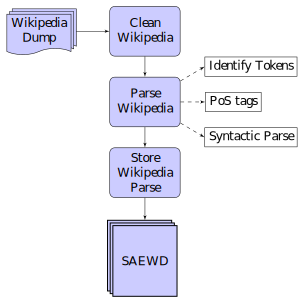
\includegraphics[scale=.8]{images/Chapitre7/flow_chart.pdf}
	\caption{The tree steps we took to build SAEWD.}
	\label{fig:flow}

\end{figure}

\section{Construction of SAEWD}
The three main steps we followed to build SAEWD are presented in Figure \ref{fig:flow}. Briefly, we have one input, which is the Wikipedia dump and one output which is the parsed snapshot. In the following we provide a detailed description of each of the process. 

 
We begin the construction of the parsed corpus with the Wikipedia dump XML file obtained from the Wikipedia database\footnote{\url{https://dumps.wikimedia.org/enwiki}} from early November 2014. This dump  contains around 4.7 million article pages\footnote{We kept all articles available in the Wikipedia dump.}. As shown in Figure \ref{fig:flow}, we apply the following processing steps in order to yield the final parsed version.
 
\subsection{Cleaning Wikipedia} First, we discard Wikipedia's  tables, references and lists, markup annotations and HTML tags with the \textit{WikiExtractor} \cite{Attardi2015}  script. 
We used this tool to clean and split the content of the original XML file into 429 folders each one containing 100 files of approximately 300 kB. These files contain a certain number of complete Wikipedia articles which is automatically determined by WikiExtractor  according to the maximum possible size assigned for each file, 300 kB in our case, thus the number of articles in each file may vary. We decided to use numerous files as well as a small size to easily read their content into memory while parsing. Having multiple small files also makes it easier to handle the multi-threading aspect of our parsing tool.
We kept WikiExtractor's original folder nomenclature which assigns to each one of them a sequence of letters sorted lexicographically\footnote{We have folders named \textit{AA}, \textit{AB}, \textit{AC} and so on.}. The files containing the cleaned text is simply named \textit{wiki\_XX} where  \textit{XX} goes from 00 to 99, as we have 100 files per folder. 
It is important to note that the Wikipedia articles' titles themselves are not sorted in any specific way, as it was not in the interest of our research to have them ordered. 
Inside each cleaned file, besides the article's text, WikiExtractor keeps the original article's URL as well as its unique Wikipedia ID within an XML-like label that also doubles as  article separator. 

\subsection{Parsing Wikipedia} Next, once the Wikipedia dump had been cleaned, we use the Stanford CoreNLP\footnote{\url{http://nlp.stanford.edu/software/corenlp.shtml}} \cite{manning2014} analysis tools to parse all the file texts produced during the previous step. As a part of our processing pipeline, we first perform  sentence segmentation, word tokenization and lemmatization. Below, we briefly describe each of the extracted attributes. We also exemplify them in detail in Section \ref{text:description}.
\begin{itemize}
\item PoS tagging: We obtain the grammatical category of each word, i.e., the part-of-speech tag, using the CoreNLP default tagger, the \textit{left3words} PoS tagging model.
\item Dependency parse: this attribute consists on an extracted tree that describes the types of grammatical relations between words, i.e., the dependency-based parse tree. 
The analysis was performed with the Stanford's \textit{Shift-Reduce}  parser.
% This parser is known to perform better than other Stanford parsers.                                  
 %(notably  faster and  with stronger \textit{F1} measure than the previous PCFG parser, although not as accurate as the Recurrent Neural Network system trained with semantic word vectors).
As information representation, we use the basic dependencies scheme, as we wanted to include each one of the possible dependency relations without any collapsing between them.    
                                                                                                                                                                                    
                                                                                                                                                                                    
\item Constituents parse:                                                                                                                                                           
the output of this analysis is a rooted tree that represents the syntactic structure of a phrase.                                                                                  
This tree is commonly known as the constituency-based parse tree.                                                                                                                  
For each word, we store its complete path in the constituency tree.
 Specifically, we keep all the nodes of a word's own branch from the root to the word itself.
 We employ the Stanford Shift-Reduce parser.
 This path is transformed into a single line and included in SAEWD. 
 

\end{itemize} 	
%\subsection{Parsed files organization}
 Finally, once the parsing process is complete, the parsed files are stored into individual files and thus there are as much parsed files as input Wikipedia cleaned files. The parsed files keep their original name plus the \texttt{parsed} extension, e.g., \texttt{wiki\_00.parsed}. The structure within the files is described in Section \ref{section3.2}. After parsing, we found the statistics shown in Table \ref{tab:corpus_stats}.
 
\begin{table}[t]
\centering
\caption{English Wikipedia dump statistics.}
\label{tab:corpus_stats}
\begin{tabular}{lr}
{\bf Number of tokens}      & 1,889,769,908 \\
{\bf Unique tokens (types)} & 8,761,691 \\
{\bf Number of sentences}   &  84,760,512\\
{\bf Average number of tokens per sentence} & 22.30
\end{tabular}
\end{table}

\section{SAEWD Description}\label{text:description}
In this section we describe in detail the characteristics of SAEWD.




\begin{table*}[ht]
\centering
\caption{Extract of a Wikipedia parsed file. The phrase shown is the parse result of the previous example sentence in Figure~\ref{fig:tree} }
\label{tab:parse}
\noindent\makebox[\textwidth]{%
\begin{tabular}{llllll}
 \multicolumn{6}{l}{\textit{FILENAME wiki\_00.parsed}}                                           \\ \hline
  \textbf{token}   & \textbf{lemma}   & \textbf{POS} & \textbf{constituency}                      & \textbf{head} & \textbf{dependency} \\ \hline
 \multicolumn{6}{l}{\textit{\%\%\#PAGE Anarchism}}                                         \\ \hline
  {$\vdots$}      &      {$\vdots$}   &  {$\vdots$}   &     {$\vdots$}                              &    {$\vdots$}  &     {$\vdots$}       \\  \hline
 \multicolumn{6}{l}{\textit{\%\%\#SEN 25  9}}                                             \\ \hline
						 A       & a       & DT  & NP\_22,S\_97                      & 3    & det        \\ %\cline{2-7} 
                         great   & great   & JJ  & NP\_22,S\_97                      & 3    & amod       \\ %\cline{2-7} 
                         brigand & brigand & NN  & NP\_22,S\_97                      & 4    & nsubj      \\ %\cline{2-7} 
                         becomes & become  & VBZ & VP\_44,S\_97                      & 0    & root       \\ %\cline{2-7} 
                         a       & a       & DT  & NP\_18,NP\_20,VP\_44,S\_97        & 6    & det        \\ %\cline{2-7} 
                         ruler   & ruler   & NN  & NP\_18,NP\_20,VP\_44,S\_97        & 4    & xcomp      \\ %\cline{2-7} 
                         of      & of      & IN  & PP\_57,NP\_20,VP\_44,S\_97        & 9    & case       \\ %\cline{2-7} 
                         a       & a       & DT  & NP\_18,PP\_57,NP\_20,VP\_44,S\_97 & 9    & det        \\ %\cline{2-7} 
                         Nation  & nation  & NN  & NP\_18,PP\_57,NP\_20,VP\_44,S\_97 & 6    & nmod       \\ %	\cline{2-7} 
\hline 
      
\end{tabular}}
\end{table*}

% Please add the following required packages to your document preamble:
% \usepackage{multirow}
% \usepackage{graphicx}
\begin{table*}[ht]
\centering
\resizebox{\textwidth}{!}{%
\begin{tabular}{cl|cccc|cccc|c}
\multirow{2}{*}{\textbf{PoS Tag}} & \multirow{2}{*}{\textbf{Token}} & \multicolumn{4}{c}{\textbf{NP}} & \multicolumn{4}{c}{\textbf{DEP}} & \multicolumn{1}{l}{\textbf{SEN}} \\ 
 &  & \multicolumn{1}{c}{$ \text{NP\_22}_1 $} & \multicolumn{1}{c}{$ \text{NP\_20}_1 $} & $ \text{NP\_18}_1  $& \multicolumn{1}{c}{$ \text{NP\_18}_2 $} & nsubj\_become & xcomp\_become & nmod\_ruler & \multicolumn{1}{c}{amod\_brigand} & \multicolumn{1}{l}{$ \text{~~S}_1 $} \\ \cline{1-11} 
\multirow{3}{*}{\textbf{NN}} & \multicolumn{1}{l|}{brigand} & 1 &  &  &  & 1 &  &  & & 1 \\
 & \multicolumn{1}{l|}{ruler} &  & 1 & 1 &  &  & 1 &  &  & 1 \\
 & \multicolumn{1}{l|}{nation} &  & 1 &  & 1&  &  & 1 &  & 1 \\ \hline
\textbf{VB} & \multicolumn{1}{l|}{becomes} &  &  &  &  &  &  &  & & 1 \\ \hline
\textbf{JJ} & \multicolumn{1}{l|}{great} & 1 &  &  &  &  &  &  & 1 & 1 \\ \hline
\end{tabular}
}
\caption{Brief example of the linguistic network incidence matrix of the previous used phrase. On the left side, as on the top, we can see the metadata we store for each word (rows) and each column (hyperedges). We omit the rest of the words from the example phrase for brevity.  }
\label{ref:incidence}
\end{table*}

\subsection{Constituency parse storage in detail}
%The  result from the constituency parse is not as straightforward to store as the other kinds of parses, i.e., the output is  a deeper tree structure than that of a dependency parse. Thus, we believe that the storage of this information in SAEWD requires a more in detail explanation. 
%In this subsection, we will describe how we stock the information concerning  the phrases' constituents. 

We will use an example to better explain the storage of the constituency-based parse tree. In Figure \ref{fig:tree} we can see the constituency parse of the phrase  \textit{A great brigand becomes a ruler of a Nation}. On the bottom of the figure, we observe the constituent's path (or branch), of the words \textit{brigand} and \textit{Nation}. As in any tree structure, each leaf node has a defined path from the root node to itself. In this example, the leaf containing the noun \textit{brigand} 
%(PoS tag \textit{NN})
 follows the bottom-up path \textit{NP22}$\rightarrow$\textit{S97}. \textit{Brigand's} parent node is a Noun Phrase (NP) node which in turn comes from the root of the tree, the Sentence node \textit{S}. We assign to each phrase chunk an identifier (22 and 97 in this case) in order to distinguish them according to their building elements as specified by the grammar rule used.
  In other words, a phrase chunk, e.g., a NP, a Verbal Phrase (VP), a Prepositional Phrase (PP), or other chunk defined by the grammar in CoreNLP, may be built from different types of PoS tags. Thus, again from Figure \ref{fig:tree}, we see that the sentence \textit{S97} is  built both from a NP and a VP chunk. 
 In a similar way, the noun phrase \textit{NP18} is produced by a determinant (DT) and a noun (NN), while  \textit{NP22} is generated by a determinant, an adjective (JJ) and a noun.
  The identification digits are obtained from the hash code that represents each chunk object inside our Java application. For each phrase-chunk tree node, we keep the last two significative figures produced by the \texttt{hashCode}\footnote{Java \texttt{hashCode} function description: \url{https://en.wikipedia.org/wiki/Java\_hashCode\%28\%29}} Java method.

\forestset{
    sn edges/.style={for tree={parent anchor=south, child anchor=north}},
    blue text/.style={for tree={text=blue!70}}}

\begin{figure}[]
\resizebox{\linewidth}{!}{%
\begin{forest} 
[S97
	[NP22 [DT [A, blue text]] [JJ [great, blue text]] [NN [brigand, blue text]]]
    [VP44 [VBZ [becomes, blue text]]
      [NP20
        [NP18 [DT [a, blue text]] [NN [ruler, blue text]]]
        [PP57 [IN [of, blue text]]
          [NP18 [DT [a, blue text]] [NN [Nation, blue text]]]]]]]
	\node [draw,fill = blue!20,text width=21em] at (1.5,-6.8) (sparse) {\textbf{brigand} (NN): NP22$\rightarrow$S97 \\ \textbf{Nation} (NN): NP18$\rightarrow$PP57$\rightarrow$NP20$\rightarrow$VP44$\rightarrow$S97};
\end{forest}
}

\caption{Constituency tree for the phrase \textit{{A great brigand becomes a ruler of a Nation}.}
% On the bottom, we can see the bottom-up path stored for the words \textit{brigand} and \textit{Nation}.
}
\label{fig:tree}
\end{figure}

 


As another example, the noun \textit{Nation} has the following bottom-up constituency path: \textit{NP18}$\rightarrow$\textit{PP57}$\rightarrow$\textit{NP20}$\rightarrow $\textit{VP44}. Indeed, the string \texttt{NP\_18,PP\_57,NP\_20,VP\_44,S\_97}, originating from the previously described path,  is the information we keep about the constituency parse for each token in the Wikipedia dump.



\subsection{Annotation scheme}\label{section3.2}
To store the parsed text we use a scheme  inspired by that used in \cite{ATSERIAS08}. The format can be considered as a regular tsv file (i.e., the entries are separated by tab spaces) with additional metadata tags. An extract from a parsed file can be observed in Table \ref{tab:parse}. 

The file includes two headers: the first one simply indicates the name of the current parse file; the second one contains the names that describe each column. The tags and columns our parsed dump contains are the following:
\begin{itemize}
\item Metadata tags:
\begin{enumerate}
\item {FILENAME}: indicates the original file used to extract the current parse, 
\item {\%\%\#PAGE}: denotes a new Wikipedia article, as well as its title, 
\item {\%\%\#SEN}: marks the beginning of a new sentence. It is followed by two integers: (1) the number of the current sentence, and (2), the number of tokens in the sentence.

\end{enumerate}

\item Parse columns for each token:
\begin{enumerate}
\item Token: the token itself,
\item Lemma: the token the canonical form,
\item POS: its part of speech tag,
\item Constituency: the bottom-up constituency path described before,
\item Head: the head index of the dependency relation the current token belongs to,
\item Constituency: the name of the grammatical relationship this token participates in as a dependent.
\end{enumerate}
\end{itemize}

Using the example phrase introduced before (Table \ref{tab:parse}), the token \textit{becomes} has \textit{become} as lemma, it is a verb, thus it has \textit{VBZ} as PoS tag, its constituency path is \textit{VP\_44,S\_97}, so it belongs to the verb phrase {VP44} which in turn comes from sentence {S97}. Finally, \textit{becomes}, being the main verb, is in this case the grammatical root of the sentence and its head is by convention determined as  zero. 

Concerning the computation time, SAEWD takes around 40 hours to be produced using a general purpose laptop (Intel i7 4700MQ with 4 cores, 8 GB and Linux Mint 17 as operative system). Most of the time is taken by the parsing step. 

We verified the consistency of the corpus built by analyzing a sample of 20 Wikipedia articles. The output of CoreNLP and the information contained in the corpus match.
